\begin{lstlisting}
from sie import *
\end{lstlisting}

\begin{lstlisting}
data=load_data('data/iris.csv')
\end{lstlisting}

\begin{lstlisting}
x_sertosa=data[data['class']=='Iris-setosa']['petal length [cm]']
\end{lstlisting}

\begin{lstlisting}
x=x_sertosa
mu=sample_mean(x)
N=len(x)
sigma=sample_deviation(x)/sqrt(N)
t_sertosa=tdist(N,mu,sigma)

print "total number of data points:",N
print "best estimate:",mu
print "uncertainty:",sigma
\end{lstlisting}

\begin{verbatim}
total number of data points: 50
best estimate: 1.464
uncertainty: 0.0245381834898
\end{verbatim}

\begin{lstlisting}
new_length=1.7
\end{lstlisting}

\begin{lstlisting}
distplot(t_sertosa,label='petal length',xlim=[1.37,1.8],
                 quartiles=[.01,0.05,.5,.95,.99],
)
ax=gca()
ax.axvline(1.7,color='r')
savefig('../../figs/z_test_iris.pdf')
\end{lstlisting}

\begin{verbatim}
<matplotlib.figure.Figure at 0x10f9d2710>\end{verbatim}

\begin{center}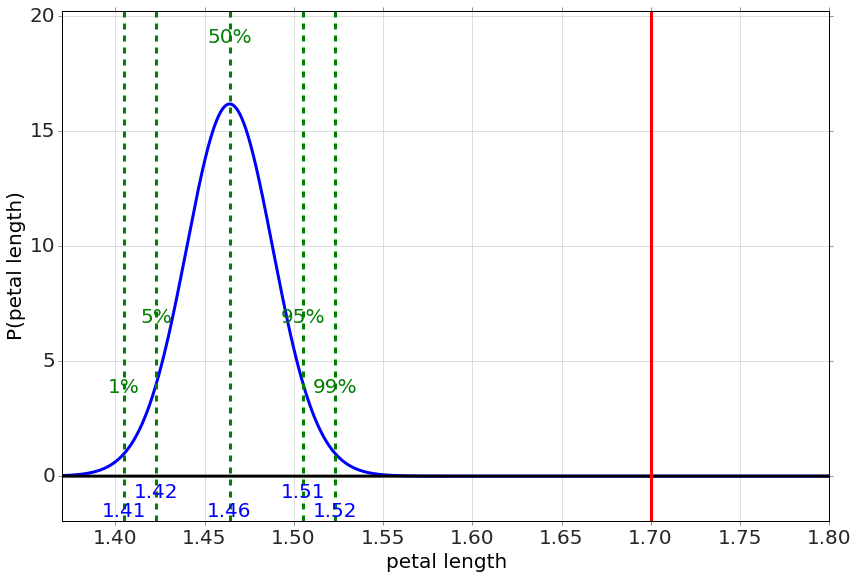
\includegraphics[width=4.5in]{Common_Significance_Tests/Common_Significance_Tests_fig0.png}\end{center}

\begin{lstlisting}

\end{lstlisting}

